\documentclass[12pt]{article}
\usepackage[paperwidth=25cm,paperheight=17cm,margin=1.5cm]{geometry}
\usepackage[T1]{fontenc}
\usepackage[utf8]{inputenc}
\usepackage[magyar]{babel}
\usepackage{lmodern}
\usepackage{amsmath}
\usepackage{enumitem}
\usepackage{tikz}
\usetikzlibrary{decorations.markings,arrows.meta}

\pagestyle{empty}
\setlength{\parindent}{0pt}
\setlist[enumerate,1]{label=\textbf{\arabic*.}, leftmargin=*, itemsep=2pt, topsep=2pt}
\setlist[enumerate,2]{label=\alph*), leftmargin=2em, itemsep=0pt, topsep=1pt, parsep=0pt}

\tikzset{
  midarrow/.style={postaction={decorate},
    decoration={markings, mark=at position 0.55 with {\arrow{Stealth[length=2.5mm]}}}}
}

\begin{document}

\begin{center}\vspace*{-0.4cm}
  {\Large\bfseries Adiabatikus folyamatok és körfolyamatok}\\[5pt]
  \fbox{\parbox{0.8\textwidth}{\centering
    Végig a $\Delta E = Q + W$ alakot használjuk, ahol $W$ a gázon végzett munka.}}
\end{center}
\vspace{-8pt}

\begin{enumerate}
\item Miért melegszik fel a biciklipumpa, amikor gyorsan pumpálunk vele? És miért
  hűl le a dezodoros flakon, amikor kifújjuk? Mindkettőt az I.~főtétellel indokold!
  Miért tekinthető egy gyors folyamat jó közelítéssel adiabatikusnak?

\item Egy gázt adiabatikusan összenyomunk. Add meg $W$, $Q$, $\Delta E$ és $\Delta T$
  előjelét, és indokold mindegyiket egy mondattal! Ugyanezt ismételd meg adiabatikus
  tágulásra is.

\item \begin{minipage}[t]{0.68\linewidth}
  Ugyanazt a gázt ugyanarról a kezdeti térfogatról ugyanakkora végtérfogatra nyomjuk
  össze, egyszer izotermikusan, egyszer adiabatikusan. Melyik esetben lesz nagyobb a
  végnyomás? Melyik esetben végzünk több munkát a gázon? Csak indokolj, számolás nélkül!
  \end{minipage}\hfill
  \begin{minipage}[t]{0.28\linewidth}\vspace{-0.7cm}\centering
  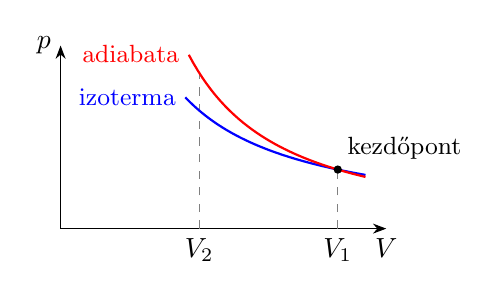
\begin{tikzpicture}[x=0.88cm,y=0.75cm]
    \draw[-{Stealth}] (0,0) -- (4.7,0) node[below] {$V$};
    \draw[-{Stealth}] (0,0) -- (0,3.1) node[left] {$p$};
    \draw[dashed,gray] (4,0) node[below,black] {$V_1$} -- (4,1);
    \draw[dashed,gray] (2,0) node[below,black] {$V_2$} -- (2,2.64);
    \draw[thick,blue,domain=1.8:4.4,samples=40] plot (\x,{4/\x});
    \draw[thick,red,domain=1.85:4.4,samples=40] plot (\x,{(4/\x)^1.4});
    \node[blue,left] at (1.8,2.22) {\small izoterma};
    \node[red,left] at (1.85,2.96) {\small adiabata};
    \fill (4,1) circle (1.5pt) node[above right] {\small kezdőpont};
  \end{tikzpicture}
  \end{minipage}

\item \begin{minipage}[t]{0.68\linewidth}
  \textbf{Fő feladat.} Egy ideális gáz a következő körfolyamatot végzi:
  $A\,(p_0, V_0) \to B\,(p_0, 2V_0)$ izobár tágulás,
  $B \to C\,(2p_0, 2V_0)$ izochor melegítés,
  $C \to D\,(2p_0, V_0)$ izobár összenyomás, végül $D \to A$ izochor hűtés.
  \begin{enumerate}
    \item Add meg szakaszonként $W$, $Q$ és $\Delta E$ előjelét!
    \item Számold ki szakaszonként a gázon végzett munkát $p_0$ és $V_0$ segítségével!
    \item Mennyi a teljes körfolyamat alatt a belső energia megváltozása? Miért?
    \item Ebből mennyi a körfolyamat alatt összesen közölt hő?
    \item Hogyan olvasható le a hasznos munka a diagramról?
  \end{enumerate}
  \end{minipage}\hfill
  \begin{minipage}[t]{0.28\linewidth}\vspace{-0.7cm}\centering
  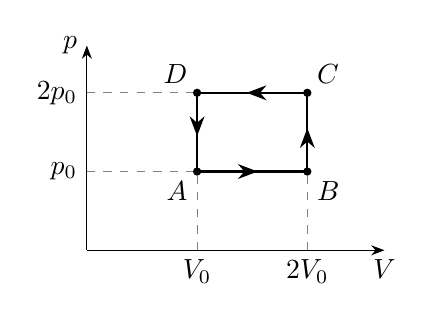
\begin{tikzpicture}[x=1.4cm,y=1.0cm]
    \draw[-{Stealth}] (0,0) -- (2.7,0) node[below] {$V$};
    \draw[-{Stealth}] (0,0) -- (0,2.6) node[left] {$p$};
    \draw[dashed,gray] (1,0) node[below,black] {$V_0$} -- (1,1);
    \draw[dashed,gray] (2,0) node[below,black] {$2V_0$} -- (2,1);
    \draw[dashed,gray] (0,1) node[left,black] {$p_0$} -- (1,1);
    \draw[dashed,gray] (0,2) node[left,black] {$2p_0$} -- (1,2);
    \draw[thick,midarrow] (1,1) -- (2,1);
    \draw[thick,midarrow] (2,1) -- (2,2);
    \draw[thick,midarrow] (2,2) -- (1,2);
    \draw[thick,midarrow] (1,2) -- (1,1);
    \foreach \p/\n/\pos in {{(1,1)}/A/below left, {(2,1)}/B/below right,
                            {(2,2)}/C/above right, {(1,2)}/D/above left}
      \fill \p circle (1.5pt) node[\pos] {$\n$};
  \end{tikzpicture}
  \end{minipage}

\item Mi változik a 4.~feladatban, ha a körfolyamatot ellenkező irányban járjuk körbe?
  Melyik mennyiségek előjele fordul meg, és melyeké nem?

\item Egy körfolyamat egyik szakasza adiabatikus tágulás. Mit tudunk erről a szakaszról
  $Q$, $W$ és $\Delta T$ szempontjából anélkül, hogy bármit számolnánk?
\end{enumerate}

\end{document}
